%======================================================================
%----------------------------------------------------------------------
%               XX                              X
%                                               X
%               XX    XXX   XXX   XXX      XXX  X  XXXX
%                X   X   X X   X X   X    X   X X X
%                X   XXXXX XXXXX XXXXX    X     X  XXX
%                X   X     X     X     XX X   X X     X
%               XXX   XXX   XXX   XXX  XX  XXX  X XXXX
%----------------------------------------------------------------------
%  	         A SKELETON FILE FOR IEEE PAPER GENERATION
%----------------------------------------------------------------------
%    Modificado por: Edgardo Vaz, Melina Rabinovich, Daniel Aicardi.  
%                                     2011                            
%======================================================================

% first, uncomment the desired options:
\documentclass[%
        %draft,
        %submission,
        %compressed,
        final,
        %
        %technote,
        %internal,
        %submitted,
        %inpress,
        %reprint,
        %
        %titlepage,
        notitlepage,
        %anonymous,
        narroweqnarray,
        inline,
        %twoside,
        ]{ieee}
%
% some standard modes are:
%
% \documentclass[draft,narroweqnarray,inline]{ieee}
% \documentclass[submission,anonymous,narroweqnarray,inline]{ieee}
% \documentclass[final,narroweqnarray,inline]{ieee}

% Use the `endfloat' package to move figures and tables to the end
% of the paper. Useful for `submission' mode.
%\usepackage {endfloat}

% Use the `times' package to use Helvetica and Times-Roman fonts
% instead of the standard Computer Modern fonts. Useful for the 
% IEEE Computer Society transactions.
% (Note: If you have the commercial package `mathtime,' it is much
% better, but the `times' package works too).
%\usepackage {times}

% In order to use the figure-defining commands in ieeefig.sty...
\usepackage{ieeefig}
\usepackage[utf8]{inputenc}


\begin{document}

%----------------------------------------------------------------------
% Title Information, Abstract and Keywords
%----------------------------------------------------------------------
\title[RF$^{2}$]{%
       Recarga Fácil por Radio Frecuencia, RF$^{2}$}

% format author this way for journal articles.
\author[D. Aicardi, M. Rabinovich, E. Vaz]{% Daniel Aicardi, Melina Rabinovich, Edgardo Vaz
	\thanks{D. Aicardi, M. Rabinovich, E. Vaz - Facultad de Ingeniería, Universidad de la República, Montevideo, Uruguay,
		{\tt\small daicav@gmail.com, mrabinovichm@gmail.com, edgardovaz@gmail.com} }
}


% specifiy the journal name
%\journal{IEEE Transactions on Something, 1997}

% Or, when the paper is a preprint, try this...
%\journal{IEEE Transactions on Something, 1997, TN\#9999.}

% Or, specify the conference place and date.
%\confplacedate{Ottawa, Canada, May 19--21, 1997}

% make the title
\maketitle               

% do the abstract
\begin{abstract}
El presente documento muestra las características de hardware y software que componen un prototipo de sistema embebido enfocado a operar con tarjetas RFID (ISO14443) como las que son utilizadas actualmente en el sistema de transporte de la ciudad de Montevideo.
\end{abstract}


% do the keywords
\begin{keywords}
Tarjetas inteligentes con y sin contacto, RFID, ISO14443, Mifare, CL RC632.
\end{keywords}

% start the main text ...
%----------------------------------------------------------------------
% SECTION I: Introduccion
%----------------------------------------------------------------------
\section{Introducción}

\PARstart El uso de tarjetas inteligentes es cada vez más frecuente en todos los ámbitos de nuestra vida cotidiana. 
Tal es el caso del sistema de transporte de la ciudad de Montevideo, donde cada pasajero utiliza una tarjeta RFID 
para efectuar el pago de cada viaje. Esto último implica que cada usuario debe cargar saldo en su tarjeta para su 
posterior uso. Es necesario entonces brindar un mecanismo simple, seguro y rápido que permita asignar saldo a cada tarjeta; la siguiente figura muestra un diagrama simplificado del sistema.

\begin{figure}[h]
\centering
  \begin{center}
  	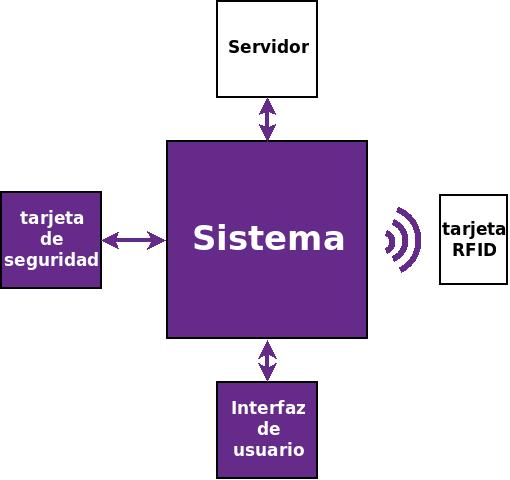
\includegraphics[scale=.3]{../pres_fin/Imagenes/diagrama_def.jpg} 
  	\caption{Bloques que conforman el sistema}\label{sist_gral} 
  \end{center}		 
\end{figure}

De los conceptos antes mencionados, se decidió implementar los bloques correspondientes al 
sistema que incluye el lector/escritor de tarjetas RFID, el lector/escritor de tarjetas 
de seguridad y la interfaz de usuario.
No fueron implementados los bloques relativos al servidor y las tarjetas RFID.


Las partes implementadas forman un prototipo de sistema embebido que interactúa con tarjetas RFID,
permitiendo consultar y/o acreditar saldo en las mismas.
El mecanismo de transferir saldo en las tarjetas RFID mediante éste dispositivo, se encuentra
desacoplado del sistema de pago de dinero, el cual podría efectuarse a través de una red de pagos,
mensajes de texto, web, etc, esto último no forma parte de este proyecto por tanto no fue implementado.



%----------------------------------------------------------------------
% SECTION II: Objetivo
%----------------------------------------------------------------------
\section{Objetivo}
El objetivo del proyecto es la fabricación de un prototipo de sistema embebido capaz de consultar y recargar tarjetas. Para ésto, como se mencionó en la introducción, deberá lograr establecer comunicación con tarjetas  como las utilizadas en el Sistema de Transporte Metropolitano (comunicación RFID a 13,56 MHz), con tarjetas de contacto (módulo de seguridad SAM), y con el usuario a través de una interfaz simple.


Esto implica entonces la fabricación de dos lectores/escritores de tarjetas, uno para tarjetas RFID (sin contacto) y
otro para tarjetas con contacto (SAM), una interfaz para el usuario capaz de informar el estado de la transacción
mediante mensajes adecuados, y la utilización de un sistema basado en un microprocesador para controlar los periféricos
y realizar las operaciones. Esto último implica además el desarrollo del software para que todo funcione adecuadamente.



%----------------------------------------------------------------------
% SECTION III: Hardware
%----------------------------------------------------------------------
\section{Hardware}
En una primera instancia se pretendía utilizar únicamente el dispositivo OpenPCD, ya que el mismo cuenta con un microcontrolador de la familia ARM, el AT91SAM7S128. Una vez estudiado se llegó a la conclusión que no permitía la instalación de un sistema operativo GNU/Linux, ya que el mismo precisa más de 4 MB de RAM para poder hacer algo útil. Otra desventaja encontrada fue que sólo tiene un puerto I2C como forma de conectar periféricos.

Surgió entonces la necesidad de usar una SBC como dispositivo capaz de ejecutar un sistema operativo y las aplicaciones necesarias para que el dispositivo cumpla con los requerimientos exigidos.

Fue necesario entonces descartar el uso del dispositivo OpenPCD y dar lugar a un diseño propio del lector/escritor de tarjetas RFID, utilizando para esto el integrado CL RC632 de Philips.

Se pensó entonces en diseñar la arquitectura que consta de SBC + lector de tarjetas RFID + lector de tarjeta de contacto + display + buzzer + leds.

En la figura \ref{Fig:HW_GRAL} se muestra un diagrama de bloques correspondiente a la arquitectura seleccionada:

\begin{figure}[h]
\centering
  \begin{center}
  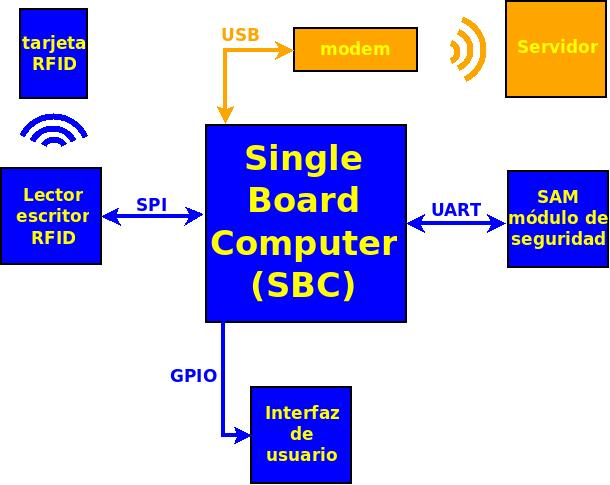
\includegraphics[scale=.3]{../docs/Imagenes/diagrama_rf2.jpg} 
  \end{center}
  \caption{Diagrama de bloques de la arquitectura seleccionada}\label{Fig:HW_GRAL} 
\end{figure}


Los bloques oscuros serán implementados, no así los claros.

La comunicación con un servidor no está implementada por quedar fuera del alcance del proyecto.

\subsection{Elección de hardware}
%\begin{itemize}
%\item SBC
\subsubsection{SBC}
En primera instancia se confeccionó una lista con posibles candidatas de SBC disponibles
en el mercado internacional, teniendo en cuenta factores como: precio, puertos de I/O, memoria RAM, memoria Flash, puertos USB, soporte para GNU/Linux, entre otros.
Se definieron una serie de requisitos mínimos necesarios para seleccionar de la lista la SBC que más se adecuara a la arquitectura definida.
Para la comunicación con el resto de los módulos será necesario: una interfaz UART para el módulo de seguridad (SAM); una interfaz SPI para el módulo lector/escritor RFID (CL RC632 de Philips); 20 GPIO para display, leds, buzzer, otros; 1 USB host previendo una futura conexión de un modem 3G (intercambio de datos con un servidor). En cuanto a la memoria disponible debe ser de 32 MB de RAM y 8 MB de flash para un funcionamiento aceptable. Es conveniente, pensando a futuro, que el procesador trabaje a una frecuencia no menor a 200 MHz.
Dado el presupuesto estimado para el proyecto, el precio no debe superar los 150 dólares en origen.
Como requisito adicional se exigió que existiera un foro actualizado y soporte técnico que permitiera evacuar dudas.

Finalmente, la SBC seleccionada para trabajar fue la Beagleboard rev.C4.

Las características generales de la BeagleBoard son: cuenta con un procesador \\
OMAP3530 de 720 MHz con arquitectura ARM. Posee  memoria NAND-flash de 256 MB y memoria ROM de igual tamaño. Tiene una ranura adicional para extender la memoria a través de una memoria SD. Entre otras cosas cuenta con un puerto USB OTG, un puerto USB host, un bloque de expansión de 28 pines (con señales a 1,8 Volt), puerto JTAG, conector RS232, etc.\\
En lo que respecta a la potencia disipada, la Beagleboard tiene un consumo de pico de 2W, y un consumo promedio de 560mW \cite{consumo1} \cite{consumo2}.

%\item 
\subsubsection{VLT - Conversor de Voltajes}
La placa de circuito impreso VLT consta básicamente de dos conectores, uno de ellos permite la conexión con la Beagleboard y el otro la conexión con el restante hardware el cual se encuentra intergrado en un PCB llamdo SCUI. Ambos conectores no se encuentran directamente interconectados entre sí a través de pistas, pues para el caso particular de Beagleboard fue necesario incorporar conversores de tensión que permitieran el traslado del nivel de tensión desde 1,8 Volt que usa esta SBC, a las tensiones con las que operan los periféricos, ya sea 3,3 o 5 Volt.


%\item 
\subsubsection{Lector de tarjeta de contacto}

Está compuesto por un conversor full duplex a half duplex el cual se encuentra conectado a uno de los puertos UART de la SBC a través del módulo VLT, que se describió en el punto anterior. Este conversor permite la transmisión de datos directamente entre la tarjeta y la SBC, sin necesidad de intercalar un ASIC para el manejo de tarjetas del tipo ISO7816. Cuenta también con un oscilador para alimentar la entrada de reloj de las tarjetas. La entrada de control (OE) del oscilador operada desde la SBC permite poner la salida de reloj en tercer estado, cosa muy útil a la hora de cumplir con la secuencia de inicialización de las tarjetas descritas en el estándar. El lector permite operar con tarjetas clase A (alimentadas a 5 Volt) y clase B (alimentadas a 3,3 Volt) haciendo uso de un jumper que permite intercambiar la tensión de alimentación suministrada a la tarjeta. Se cuenta con un zócalo para insertar la tarjeta de contacto.


%\item 
\subsubsection{Interfaz de usuario}

Está compuesta por tres leds (verde, amarillo y rojo), buzzer y un display LCD16x2 donde son desplegados los mensajes que indican al usuario la operación que se efectúa sobre su tarjeta Mifare.


%\item 
\subsubsection{Lector de tarjetas RFID}

Este módulo es el encargado de la comunicación con las tarjetas RFID que cumplen con la norma ISO14443. Consta básicamente de cuatro secciones entre las que se encuentran: el integrado CL RC632; el filtro EMC, el circuito de adaptación de impedancia (matching); y el inductor de la antena. 
El ASIC CL RC632 permite, por un lado la comunicación digital con un microprocesador a través de su puerto de datos y por el otro lado la transmisión de datos hacia la antena que emitirá la señal RF para la comunicación con las tarjetas ISO14443.

Lo que se llama propiamente antena RF está conformada por el circuito de adaptación de impedancia (matching) y por el inductor ubicado en el circuito impreso, que propaga el campo magnético para lograr el acoplamiento necesario entre lector y tarjeta, de aquí la sigla PCD (Proximity Coupling Device).
%\end{itemize}



%----------------------------------------------------------------------
% SECTION IV: Software
%----------------------------------------------------------------------
\section{Software}

\subsection{Introducción}
Se debe destacar que todo el desarrollo de software se basó exclusivamente en herramientas de software libre. La distribución GNU/Linux elegida para el sistema embebido se llama Angström. Esta distribución es muy usada en aplicaciones que utilizan una Beagleboard como SBC y cuenta con una gran cantidad de bibliotecas implementadas en lenguaje C, que permiten gran escalabilidad a la hora de incorporar nuevos periféricos en la aplicación.


\subsubsection{Sistema Operativo}
En el arranque, la Beagleboard tiene la posibilidad de buscar el bootloader y el kernel en NAND, o en dispositivos extraíbles tales como memorias USB o memorias SD. Para el sistema RF$^{2}$, se eligió un arranque a través de una memoria SD ya que es fácil de manipular.

En la figura \ref{Fig:SD} se puede ver como queda distribuida la memoria SD con las distintas partes
que conforman el sistema operativo. 

\begin{figure}[h]
\centering
  \begin{center}
  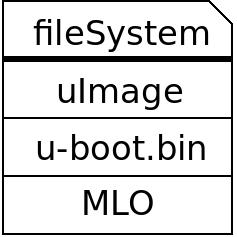
\includegraphics[scale=.4]{../docs/Imagenes/sd.jpg} 
  \end{center}
  \caption{Memoria SD para funcionar en Beagleboard}\label{Fig:SD} 
\end{figure}

En la memoria SD se pueden distinguir dos particiones, una en formato FAT32 y otra
en formato ext3. La partición en FAT32 es llamada “de arranque”, y es donde se encuentra 
el bootloader (MLO, u-boot.bin) y la imagen comprimida del kernel (uImage). 
La partición en ext3 es donde se encuentra el sistema de archivos (fileSystem) asociado con la distribución elegida.

%El MLO es el equivalente al bootloader de la primera etapa, en general ya viene precargado en la memoria NAND de la Beagleboard. Es posible generarlo, o incluso bajar una versión ya compilada desde la web de Angström. Como característica principal tiene la capacidad de buscar el u-boot.bin en dispositivos extraíbles como memorias SD o USB.
%
%El u-boot.bin es equivalente al bootloader de la segunda etapa. En el sistema RF$^{2}$ fue necesario generarlo, ya que tiene la posibilidad de configurar el bloque de expansión de la Beagleboard.
%
%El uImage es el kernel comprimido del sistema. Fue necesario generarlo, ya que se debieron modificar sus fuentes para que queden habilitadas las interfaces de comunicación con los dispositivos periféricos.
%
%El fileSystem (también conocido como RootFileSystem) es el correspondiente a una distribución GNU/Linux llamada Angström. Se pueden llegar a precargar distintos programas y bibliotecas dependiendo de la forma en que se genere.
%Angström es una distribución GNU/Linux diseñada específicamente para sistemas embebidos desarrollados
%para SBCs como la usada para este prototipo. Ésto lo hace más eficiente que otros sistemas operativos para la aplicación desarrollada. La elección de esta distribución se debió a que es de los más recomendados y utilizados en la documentación y foros de Beagleboard.


\subsection{Herramientas utilizadas en el desarrollo del sistema}

\subsubsection{Introducción}
Para el desarrollo de sistemas existe una gran variedad de herramientas útiles, algunas de software libre y otras privativas. El hecho de tener tantas opciones disponibles, a pesar de ser una ventaja, a veces dificulta la elección de las herramientas correctas.

Para la elección de las herramientas se tomó como primer criterio de decisión el hecho que sean libres, así como las experiencias de otras personas que ya han transitado caminos comunes, consultando y participando en foros activos.


A continuación se detallan algunas de las herramientas utilizadas para el desarrollo del sistema. 

\subsubsection{MLO, u-boot.bin y uImage}
No fue necesario generar el MLO debido a su simpleza, puesto que el binario precompilado realiza bien su función.

El u-boot.bin y el uImage fueron generados con la herramienta de desarrollo y compilación OpenEmbedded-Bitbake que es una fusión de dos herramientas: OpenEmbedded, herramienta para construcción y mantenimiento de distribuciones, y Bitbake, herramienta de compilación similar al Make que automatiza la construcción de ejecutables entre otros. Esto es, OpenEmbedded utiliza Bitbake para su objetivo. OpenEmbedded-Bitbake es una herramienta muy potente y difícil de aprender al principio. Luego de entendido su principio de funcionamiento se hace muy simple su uso.
% para lo que es necesario tener acceso a una buena conexión a internet debido a que realiza descargas de paquetes en forma habitual.
%Con esta herramienta también se pueden generar el MLO y el fileSystem, aunque se prefirió utilizar otras herramientas por sobre ésta. 
%Su instalación, configuración, estructura y uso se pueden ver en el apéndice.

\subsubsection{FileSystem}
Para la generación del fileSystem de Angström, se utilizó la herramienta web Narcissus disponible en la página de Angström.
%Esta herramienta permite seleccionar entre diferentes dispositivos (entre los cuales está Beagleboard), los programas que se quieran instalar, el formato de la imagen seleccionada, e incluso se puede generar un kit de desarrollo (SDK) para el PC de desarrollo. Debido a la facilidad de uso y a los buenos resultados obtenidos, se decidió utilizar esta opción por sobre la del fileSystem generado por la herramienta OpenEmbedded-Bitbake.

\subsubsection{Crosscompilación}
Se llama crosscompilar al proceso de compilación en una arquitectura, generando binarios para su ejecución una arquitectura diferente. En el caso del proyecto RF$^{2}$, se compilan paquetes en una arquitectura x86 (PC de desarrollo) para ser utilizados en una arquitectura ARM.

Para la crosscompilación se utilizó el SDK generado por Narcissus y la herramienta Make para generar los archivos necesarios.

\subsubsection{Depuración de código}
Para la depuración, se utilizó la herramienta GDB del proyecto GNU. 


\subsubsection{Bibliotecas}

\begin{itemize}
\item pcsc-scan 
%es una herramienta de uso por línea de comandos, que una vez ejecutado imprime el nombre del lector PC/SC conectado y en caso que exista una tarjeta de contacto insertada imprime también su ATR. Luego  escanea el lector constantemente e indica si se retira o inserta una tarjeta. 
Esta aplicación fue utilizada para testear el lector de tarjetas de contacto.
\item  librfid-tool 
%es una herramienta de uso por línea de comandos que da acceso de bajo nivel RFID utilizando los lectores soportados por la biblioteca para manejo de lectores/escritores RFID, librfid. 
Esta herramienta fue utilizada para testear lectores/escritores de tarjetas RFID.
\end{itemize}


\subsection{Desarrollo}

\subsubsection{MLO}
Como se mencionó anteriormente, no fue necesario generar el MLO debido a que la Beagleboard viene con uno pre-instalado, y en caso que no funcione en forma correcta se puede descargar desde un repositorio de Angström. No fue necesario realizar ningún cambio en el archivo ya que realiza su función correctamente.

\subsubsection{Multiplexado de pines}
El microprocesador OMAP3530 tiene muchos pines con distintas interfaces entre las
que se cuentan puertos UART, SPI, GPIO, etc., pero no todos son accecibles desde la Beagleboard. 
Para poder acceder a algunos de estos puertos del microprocesador, existe en la placa de la
Beagleboard un bloque de expansión de 28 pines.


Por defecto, en el bloque de expansión no se encuentran las señales que se quieren. Esto 
lleva a que se tenga que modificar el estado inicial de los pines. 
Existen dos formas de modificar los pines de modo de tener las señales que se precisan. Una de ellas es modificar el bootloader y la otra es modificar el kernel. Esto implica cambios en los archivos fuentes y posterior compilación que genere los nuevos binarios u-boot o uImage. 


Para la modificación de las señales disponibles en el bloque de expansión se decidió modificar el u-boot, ya que la modificación por u-boot es más intuitiva y por experiencia se sabe que lo que más se actualiza y/o modifica es el kernel. 

\subsubsection{u-boot}
Como se mencionó anteriormente, en el u-boot se realizó la configuración de los pines del bloque de expansión de la Beagleboard. 
Cada pin del bloque de expansión tiene varias funcionalidades asociadas, y la configuración de la 
funcionalidad depende de un multiplexado modificable a nivel de software. Esto es, dependiendo del “modo de pin” elegido, la función que se obtiene en dicho pin.
%Para que los cambios hechos en el u-boot tengan el efecto esperado al arrancar el sistema, es necesario que en la configuración del kernel esté la opción CONFIG\_OMAP\_MUX=no, lo que imposibilita al kernel a realizar este mismo cambio. Esta opción no está activada por defecto para versiones de kernel 2.6.32 y posteriores. 
%

%Antes que pueda ser modificado el estado de los pines del bloque de expansión,
%es necesario obtener los archivos fuente con los cuales se genera el archivo binario u-boot.
%
%En el apéndice \ref{anx_sw_ub} se encuentran los pasos a seguir para generar el archivo binario u-boot.bin.
%

%El archivo generado se encuentra en /stuff/build/tmp/deploy/glibc/images/beagleboard/ aunque con su nombre seguido de un número identificatorio, el cual debe ser borrado para poder mantener el nombre necesario (u-boot.bin).


Pese a que en la literatura y foros, se plantea lo contrario, no fue posible establecer los atributos “valor” y “dirección” de los pines GPIO mediante la modificación planteada. Lo que sí cambia efectivamente es el modo del pin, permitiendo obtener las interfaces adecuadas en el bloque de expansión.

\subsubsection{uImage}
La versión del kernel elegida fue la 2.6.32 ya que en el momento que se comenzó el desarrollo era la versión más estable.
%Durante el arranque del sistema, el kernel carga los módulos y controladores necesarios para el funcionamiento del 
%hardware que forma parte del sistema embebido. También se montan las interfaces para poder interactuar con los distintos dispositivos a ser conectados a la Beagleboard como lo son: SPI, GPIO, UART, etc.. Las interfaces SPI y UART se encuentran bajo el directorio /dev en el sistema de archivos, y GPIO bajo el directorio /sys/class/gpio. 
En algunos casos, 
%en /dev 
no aparecen algunas de las interfaces configuradas, lo que lleva a modificar los fuentes del kernel para que esto así suceda. Este fue el caso de la interfaz SPI que no quedó mapeada en /dev pese a que había sido configurada en los fuentes del u-boot. También hubo problemas con los atributos “valor” y “dirección” de los GPIO, como se mencionó anteriormente. Adicionalmente hacía falta un módulo para simular una conexión ethernet sobre una interfaz USB para establecer una conexión entre la Beagleboard y un PC, que emula una tarjeta de red por software.
Todo esto llevó a que se tuvieran que modificar los archivos fuente del kernel.

\subsubsection{FileSystem}

Como se mencionó anteriormente, el fileSystem se generó a partir de la herramienta web Narcissus.\\
En el fileSystem es donde se encuentran los paquetes y programas ya instalados. Cuanto más programas se instalen más grande será en tamaño el fileSystem.

%seccion 6.4.7
\subsubsection{Bibliotecas}

\leftline{\bf{Software para el manejo de GPIO}}

Este módulo de software fue realizado desde cero, basándose en el fileSystem virtual SYSFS para el control de GPIOs \cite{gpio} \cite{gpioK}, esto permite que el código pueda ser portado a cualquier otro sistema que use GNU/Linux y que disponga de este tipo de hardware.


%El módulo de software para el uso de los puertos de propósito general, GPIO, en principio puede resultar poco importante a simple vista, pero esta porción de código es usada por el resto de los módulos que conforman la aplicación completa del prototipo RF$^{2}$. 
%Este módulo cuenta básicamente con una estructura que permite almacenar el estado de cada puerto, una macro, y cuatro funciones que se datallan a continuación.
%La primera de las funciones se llama config\_gpio\_pin() y permite exportar desde el espacio kernel al espacio usuario las funcionalidades necesarias para hacer uso del puerto que se indica como argumento. Al momento en que se exporta, se indica la dirección, o sea si será un puerto de entrada o salida, a través de un parámetro que es pasado a la función.
%La función que permite leer el valor actual de un puerto se llama read\_gpio\_pin(), es necesario pasarle como argumento el indicador del puerto del cual se quiere conocer su valor. El valor del puerto es guardado en la estructura que almacena el estado de cada puerto para posteriores consultas, sin tener que volver a llamar a dicha función.
%Las últimas dos funciones son contrapuestas, set\_gpio\_pin() y clear\_gpio\_pin(), éstas permiten poner el valor de un puerto específico en el valor lógico “1” o “0” respectivamente. Previo a establecer o borrar el valor del puerto ambas funciones verifican que la dirección del mismo sea de salida (como mecanismo de seguridad no es posible cambiar el valor de un puerto de entrada).
%Por su parte la macro reset\_status\_gpio() permite borrar el estado de un puerto que ya no esté en uso.



\leftline{\bf{Software para comunicación SAM}}

Hoy en día la mayoría de los lectores de tarjetas de contacto tienen una interfaz USB para ser conectado en un PC en aplicaciones de escritorio. Para el uso de este tipo de lectores sobre GNU/Linux, se hace uso de la especificación USB llamada CCID.
Sin embargo, las tarjetas de contacto no poseen un puerto USB sino un puerto serie para establecer la comunicación con algún dispositivo, es por esto que en la nueva generación de lectores siempre hay un ASIC para lograr la interacción, por un lado con la tarjeta de contacto y por el otro la comunicación con el PC.
Como fue descrito en la sección de hardware, el lector de tarjetas de contacto tiene una interfaz serial pura para la transferencia de datos con las tarjetas. En base al diseño hardware elegido, las capas de software sobre las que se decidió trabajar son las que se detallan en la figura \ref{Fig:capas}. 

\begin{figure}[h]
\centering
  \begin{center}
  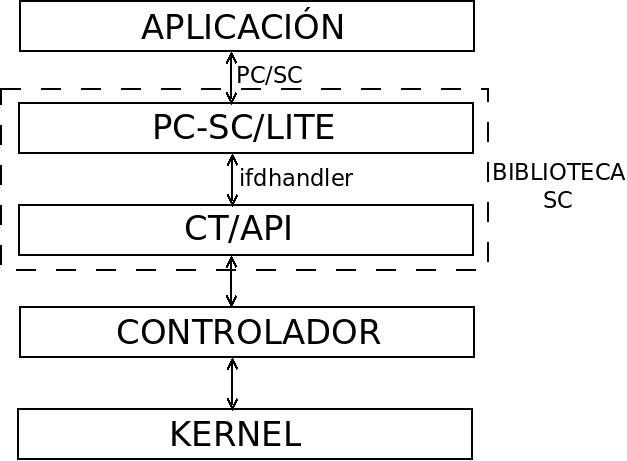
\includegraphics[scale=.35]{../docs/Imagenes/SW_sc1.jpg} 
  \end{center}
  \caption{Capas de software de trabajo}\label{Fig:capas} 
\end{figure}


%En una primera etapa y para simplificar el desarrollo y la depuración del software, las capas empleadas fueron las que se muestran en la figura \ref{Fig:capas0}.
%
%
%\begin{figure}[h]
%\centering
%  \begin{center}
%  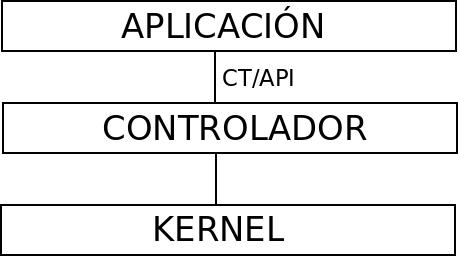
\includegraphics[scale=.4]{../docs/Imagenes/SW_sc2.jpg} 
%  \end{center}
%  \caption{Capas de software en una primera etapa}\label{Fig:capas0} 
%\end{figure}


A continuación se describen las capas asociadas a la figura \ref{Fig:capas}.


\leftline{Controlador:}
El kernel es el encargado de manipular directamente los registros del puerto serial, las interrupciones que desde éste se generan y la ISR para atender las interrupciones.
La implementación del controlador del lector de tarjetas se basó en el controlador serial de GNU/Linux a través de su estructura “termios” \cite{termios}. Esta estructura permite configurar todos los parámetros necesarios para la comunicación serial como ser, baud rate, cantidad de bits por byte, bit de paridad, bit de parada entre otros. Las funciones read y write permiten la lectura y escritura de los bytes de datos que son recibidos y transmitidos por el puerto serial.

%Dentro del proyecto MUSCLE/PCSCLite existe código ejemplo de controladores de lectores de tarjetas de contacto que son compatibles con la biblioteca, si bien el desarrollo se basó en alguno de ellos, como el hecho de usar el mismo nombre de funciones, su contenido fue desarrollado específicamente para controlar el hardware específico del prototipo RF$^{2}$.


CT/API (Card Terminal / Application Programming Interface):
Por encima del controlador serial se encuentra CT/API \cite{ctapi}, una interfaz definida por varias empresas (entre las que se incluye Telekom Alemania) en la década de los noventa, que permite encapsular el controlador específico de cada lector de tarjetas, de manera que la aplicación final no se vea afectada al cambiar un lector por otro.
Esta interfaz de programación está formada tan solo por tres funciones, CT\_init, CT\_data y CT\_close, que permiten la inicialización del lector, la transferencia de datos entre \\
host/lector o host/tarjeta (host se refiere a la SBC o PC donde se encuentra conectado el lector de tarjetas de contacto) directamente y el cierre de la comunicación.\\
%CT\_init se encarga del pasaje de parámetros a la capa del controlador, para la configuración del puerto de comunicación entre el host y el lector de tarjetas. Los parámetros en uso aquí son: la tasa de transferencia de datos, el número de bits por cada byte, el tipo de paridad empleado y el puerto serie a ser utilizado.\\
%CT\_data es la función encargada de transferir comandos y datos hacia y desde la tarjeta o hacia y desde el lector (en caso que el mismo esté formado por un ASIC o microprocesador). La manera de diferenciar desde donde es enviado el dato, es a través de un parámetro pasado a esta función, y de forma análoga se determina el destino del mensaje. El protocolo usado para la transferencia de datos es T=0, orientado a bytes y del cual pueden conocerse más detalles en \cite{SCHb}.\\
%CT\_close es la contracara de  CT\_init, se encarga de cerrar la comunicación con el lector. Lo que hace básicamente es liberar el handle (puntero) asociado al puerto serial.
%
%Las funciones de apertura y cierre de la comunicación no necesitan ser modificadas, son similares en todos 
%los controladores de lectores seriales compatibles con la biblioteca. Por otro lado la función CT\_data debió ser sustancialmente modificada para lograr el intercambio de datos a partir del protocolo T=0.
%

%Para el caso en que los comandos y/o datos estén dirigidos hacia el lector, existe otra especificación, llamada CT/BCS \cite{ctbcs} (Card Terminal / Basic Command Set), donde se encuentran definidos una serie de comandos básicos para el manejo del lector. Estos comandos se nombran a continuación y se da una breve descripción.
%

%RESET CT permite reiniciar el lector o tarjeta (en el caso de ser un lector mudo); de manera opcional puede devolver el ATR.
%
%REQUEST ICC tiene como objeto devolver el ATR de la tarjeta una vez que la misma se encuentra ubicada en el zócalo del lector.
%
%GET STATUS es empleado para conocer información sobre el lector o si la tarjeta está insertada y eléctricamente conectada en el lector. 
%
%EJECT ICC genera la desactivación eléctrica de la tarjeta.


\leftline{IFDHandler:}
El siguiente componente en este stack de capas es ifdhandler; no es otra cosa que un conjunto de funciones formando una API, empleada por pcsclite para encapsular el manejo del hardware de lectores cuyos fabricantes quieran cumplir con las especificaciones PC/SC. Una ventaja importante de esta API es que le permite a pcsclite operar tanto con lectores de puerto serial como con lectores de puerto USB.
Esta capa de software podría usarse directamente sobre el controlador del lector, prescindiendo de CT/API, aunque se decidió mantenerla por motivos de simplicidad ya que sólo es necesario sustituir la capa de aplicación por las restantes capas superiores como se indica en la figura \ref{Fig:capas}.


Las funciones que contiene esta capa de software fueron modificadas para que contengan a su vez las funciones de CT/API, y de esta manera hacer más fácil de integrar el controlador del lector con la biblioteca PCSCLite.


%En lo que sigue se enumeran algunas de las funciones de esta API y se describen brevemente. Por más detalles ver el manual ifdhandler \cite{ifdhandler}.
%

%IFDHCreateChannel establece el canal de comunicación con el lector. Para conseguirlo usa un parámetro llamado Channel, que indica cual es el puerto serial a usar, por ejemplo para el caso de GNU/Linux /dev/ttySx (x es el número que corresponda).
%
%IFDHCloseChannel implementa la acción opuesta a la función anterior, cerrando el canal de comunicación con el lector de tarjetas.
%
%IFDHGetCapabilities permite obtener las capacidades específicas del lector o de la tarjeta insertada en el mismo.
%
%IFDHPowerICC se encarga del control de las señales de alimentación y reset que el lector suministra a la tarjeta. Desempeña tres acciones posibles, encendido, reset y apagado de la tarjeta.
%
%IFDHTransmitToICC se encarga de la transferencia de datos con la tarjeta a través de alguno de los protocolos disponibles, como ser T=0 o T=1.
%
%IFDHICCPresence retorna el estado de la tarjeta insertada en el zócalo del lector.


\leftline{PCSCLite:}
Por arriba de ifdhandler se encuentra la biblioteca pcsclite, ésta contiente todas las funciones necesarias para establecer la comunicación con un lector y la tarjeta conectada a éste último.
%Para el uso del controlador encapsulado por ifdhandler desde pcsclite es necesario seguir los pasos de configuración detallados en el apéndice \ref{anx_pcsc_inst}.


\leftline{Aplicación final:}
Por arriba de todas las capas descritas antes, se encuentra la aplicación del prototipo que hace uso de las funciones suministradas por pcsclite y donde se encuentran definidos los comandos APDU específicos con los que opera la tarjeta de contacto.
%Por razones de seguridad no se nos permite difundir la lista de comandos que son usados para la comunicación con el módulo SAM.


\leftline{\bf{Software RFID}}
librfid es una biblioteca de software libre para manejo de lectores/escritores RFID. Implementa el stack de protocolos del lado del dispositivo lector/escritor ISO 14443A, ISO 14443B, ISO 15693, Mifare Ultralight y Mifare Classic.

Entre los lectores soportados están, OpenPCD y algunos modelos Omnikey, éstos con interfaz de conexión USB. Además tiene soporte para cualquier otro lector con comunicación directa con el CL RC632 mediante la interfaz SPI y es por esta razón que se tuvo en cuenta.

El manejo de librfid es de bajo nivel y se comunica directamente con el kernel utilizando el módulo spidev. Librfid-tool implementa funciones de más alto nivel que hacen uso de las funciones de bajo nivel de la librfid. La estrucrura de software comentada se muestra en la figura \ref{sw_RFID}.

\begin{figure}[h]
\centering
  \begin{center}
  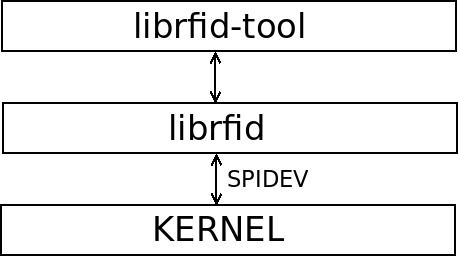
\includegraphics[scale=.4]{../docs/Imagenes/librfid-tool.jpg} 
  \end{center}
  \caption{Capa de software RFID}\label{sw_RFID} 
\end{figure}


%A continuación se detallan los cambios introducidos en la biblioteca librfid para el correcto funcionamiento del lector/escritor RFID utilizando librfid-tool.


%Se analizó el código principal de la aplicación librfid-tool y se vio que dentro del directorio utils en el archivo common.c se encuentra la función reader\_init la cual busca un lector/escritor entre los soportados. Esta función no tenía implementada una búsqueda para dispositivos conectados por SPI. Por lo tanto se tuvieron que agregar las siguientes líneas a la función para que el funcionamiento fuera posible:
%
%\begin{verbatim}
%rh = rfid_reader_open("/dev/spidev3.0", RFID_READER_SPIDEV);
%if (!rh) {
%    fprintf(stderr, "No SPIDEV found\n");
%    return -1;
%}
%\end{verbatim}
%
%Este cambio permitió detectar la interfaz SPI (spidev3.0). Algo a tener en cuenta, es que como en GNU/Linux las interfaces están asociadas a un archivo, el hecho de abrir el archivo no implica que haya nada conectado en esa interfaz. Por esta razón, la búsqueda de un lector/escritor conectado por interfaz SPI se realiza en última instancia.
%

%Otro cambio fundamental es en la frecuencia de reloj del puerto SPI. Se incrementa a 10 MHz, ya que con la frecuencia establecida por defecto en la biblioteca librfid (1 MHz) el lector/escritor RFID no funciona correctamente. 
%
%Toda la configuración de la comunicación por SPI se encuentra en rfid\_reader\_spidev.c que está en el directorio fuente src.
%
%La función que se modificó es spidev\_open y el cambio se muestra a continuación:
%
%\begin{verbatim}
%tmp = 10e6; /* 10 MHz */
%if (ioctl(spidev_fd, SPI_IOC_WR_MAX_SPEED_HZ, &tmp) < 0)
%    goto out_rath;
%\end{verbatim}
%
%Se implementaron las funciones adecuadas para el manejo del pin RST\_RF, el cual puede encender y apagar el lector/escritor RFID diseñado.


Después de estudiadas las funciones que provee la herramienta librfid-tool, se estudió la posibilidad de su uso para la aplicación RF$^{2}$. 

Aunque sus funciones  son muy útiles, la gran mayoría no sirven completamente para la aplicación RF$^{2}$ debido a que fueron definidas para otros propósitos. 

Es de interés, que la herramienta librfid-tool siga manteniendo sus funcionalidades y pueda convivir con la aplicación RF$^{2}$, por lo que no se modificó el contenido de ninguna función de la herramienta. En el caso que alguna función fuera mayormente utilizable, se procedió a crear una nueva con los cambios necesarios.

Se implementaron la mayoría de las funciones, logrando compatibilidad con la biblioteca librfid. Entre las funciones creadas están las asociadas con la tarjeta RFID: autenticación según el tipo de clave, búsqueda de tarjetas próximas al lector, lectura y escritura de bloques de memoria, obtención del UID, etc.

\subsubsection{Aplicación final}

Para el desarrollo de la aplicación RF$^{2}$ se decidió trabajar sobre los fuentes de la herramienta librfid-tool, ya que maneja varias funciones de utilidad y es de ayuda a la hora de compilar para el armado de una aplicación completa. Se mantuvieron todas las opciones de la herramienta ya que son útiles, y pueden ayudar en un futuro para establecer orígenes de fallas. No se modificó ninguna función de la aplicación original y cuando fue necesaria alguna modificación, se procedió a implementar una nueva.

En la figura \ref{Fig:SW} se detallan las capas de software del sistema RF$^{2}$.

\begin{figure}[h]
\centering
  \begin{center}
  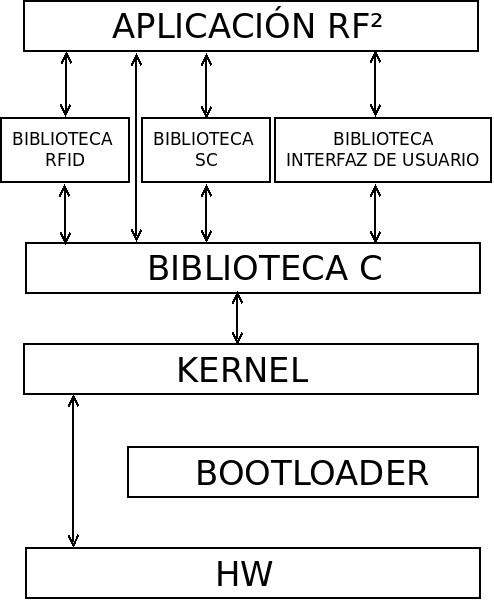
\includegraphics[scale=.35]{../docs/Imagenes/SW.jpg} 
  \end{center}
  \caption{Capas de software del sistema RF${^{2}}$}\label{Fig:SW} 
\end{figure}


%Antes de seguir fue necesario entender el funcionamiento de las reglas de compilación creadas para la aplicación librfid-tool sobre librfid. En el directorio raíz, se encuentran los siguientes archivos importantes para el desarrollo del sistema: autogen.sh, configure.in, configure, Makefile.am, Makefile.flags.am, Makefile.in, Makefile.
%

%Por detalles sobre la utilidad de cada uno de estos archivos, y su modificación para el funcionamiento de la aplicación RF$ ^{2} $ referirse al apéndice \ref{makefile}.


\leftline{\bf{Modificaciones en librfid-tool}}

Se implementó una función de inicialización, la cual inicializa todos los periféricos al arrancar la aplicación RF$^{2}$.

En librfid-tool.h se definieron constantes simbólicas para hacer configurable al sistema. 
%Algunas de ellas son:
%

%MONEDERO: lugar del arreglo “bloque” donde se encuentra el monedero.
%
%SECTOR\_MONEDERO: sector donde se encuentra el monedero.
%
%BLOQUE\_MONEDERO: bloque donde se encuentra el monedero.
%
%BLOQUE\_RESPALDO: bloque donde se encuentra el respaldo del saldo.
%
%TIEMPO\_BUZZER: tiempo de encendido del buzzer en $\mu$s.
%
%PAUSA\_BUZZER: tiempo entre dos encendidas del buzzer en $\mu$s.
%
%TIEMPO\_LED: tiempo de encendido del led en s.
%
%INICIO: tiempo de espera al inicio en s. 
%
%ESPERA: tiempo de espera estándar en s. 
%
%FIN: tiempo de espera al final en s.
%


Se agregó una nueva opción (n) en el main de la aplicación librfid-tool que llama a la función principal(). Ésta, es la función principal de la aplicación RF$^{2}$, la cual se ejecuta en loop.
% y se basa en el diagrama de flujo de la figura \ref{Fig:HW}. 
De este modo no se modifica el main original de librfid-tool (sólo se agrega la opción n) y se dejan las opciones por defecto.
Se hizo uso de algunas funciones ya escritas y se crearon otras. En este punto no se modificó ninguna función de la aplicación original y cuando fue necesaria alguna modificación, se procedió a implementar una nueva función con las modificaciones previstas.
%Luego viene la etapa de crosscompilación de la aplicación para ser probada en la SBC.
%

%Por detalles sobre la crosscompilación de la aplicación final referirse al apéndice \ref{crosap}


\leftline{\bf{Funcionamiento general de la aplicación}}

%La aplicación se desarrolló en base a los casos de uso que se indican en la figura \ref{Fig:DiagFlujo}.
Se desarrolló una estructura de directorios de forma que el sistema sea modular, esto es, cualquier cambio requerido en algún módulo del sistema, no afecta al resto.


%Los mensajes al display, se realizan mediante la función dato\_lcd() la cual despliega el mensaje adecuado según una lista de mensajes guardados en mensajes.h, dentro del directorio lcd (ver figura \ref{est_RF2}). Las funciones encender\_bl() y apagar\_bl() que se encuentran dentro del directorio lcd sirven para encender y apagar el backlight del display.
%Las funciones relacionadas a los leds y el buzzer, se encuentran en el directorio gpio (ver figura \ref{est_RF2}) y el nombre del pin asociado con el led o buzzer a utilizar se encuentra en el archivo beagle\_gpio.h dentro del directorio gpio. Las funciones lb\_error(), lb\_consulta() y lb\_recarga(), realizan el encendido y apagado adecuado de los leds y buzzer de acuerdo a si se produce un error, consulta o recarga durante la transacción en curso.
% 

%Al iniciar la aplicación, se realiza la inicialización de los distintos módulos que conforman el sistema (interfaz de usuario y habilitación de comunicación con módulo\\
% lector/escritor RFID, pin RST\_RF). Ésto se realiza mediante la función inicio\_rf2(). Luego se abre el puerto de comunicación con el lector/escritor RFID. Con estos pasos finaliza la inicialización del sistema y se ingresa al loop principal de la aplicación.
%Durante el transcurso de la transacción, se despliegan los mensajes adecuados a través de la interfaz de usuario.
%Se realiza la búsqueda de una tarjeta mediante la utilización de la función busqueda\_tarjeta() que queda en loop esperando a que se encuentre una tarjeta en el campo del lector/escritor RFID.
%Cuando se detecta una tarjeta, se inicia la comunicación con ésta mediante el uso de las funciones l2\_init() y l3\_init() (se inicia algoritmo de anticolisión y se establece el protocolo). Se previó el hecho que suceda algún error en estos pasos, volviendo a iniciar la comunicación.
%Ya establecida la comunicación con la tarjeta, se obtiene el identificador de la tarjeta sin contacto (UID). Lo anterior se realiza mediante la función obtener\_uid(). En caso de presentarse un error, se comienza nuevamente el diálogo con la tarjeta. Cuando la tarjeta no pertenezca al grupo de tarjetas habilitadas para la aplicación, se ignora la presencia de la tarjeta inválida y no se despliegan mensajes al usuario.
%Luego, se obtienen las claves asociadas con la tarjeta mediante el uso de la función claves\_mifare(). Esta función simula la comunicación con la tarjeta de contacto, la cual es la
%encargada de derivar las claves de la tarjeta RFID identificada con el UID
%obtenido en el paso anterior. Dado que es una función asociada con la tarjeta de contacto, ésta está definida en el archivo sam.c dentro del directorio sam (ver figura \ref{est_RF2}).
%Resta averiguar si la tarjeta tiene saldo a acreditar o no. Para ésto se utiliza la función consulta\_recarga(), la cual devuelve el monto a recargar a partir de la lectura del archivo local carga.txt. Para que el dispositivo no funcione en forma local la consulta de las opciones de recarga se hacen contra un servidor, como se indicó anteriormente esto no fue implementado por estar fuera del alcance de este proyecto.
%
%A partir de aquí se diferencian dos casos, si la función anterior devuelve un valor mayor que cero entonces se está frente a una recarga, si devuelve cero, se está frente a una consulta. Si devolviera un valor negativo (por algún tipo de error) se realiza una consulta.
%
%En el caso de consulta, se utiliza la función consulta, la cual con las claves adecuadas, lee el contenido de la memoria de la tarjeta asociado con el monto actual (Monedero) y despliega los mensajes adecuados mediante la interfaz de usuario.
%
%En el caso de recarga, se hace uso de la función recarga, la cual con las claves adecuadas, lee el contenido de la memoria de la tarjeta asociado con el monto actual (Monedero), lo respalda (Respaldo), luego calcula el nuevo saldo, y escribe el nuevo saldo en el Monedero. Durante este proceso se despliegan los mensajes adecuados mediante la interfaz de usuario. Si la recarga se realizó correctamente, se debe borrar el saldo a acreditar obtenido mediante consulta\_recarga() (para no cargar dos veces el mismo saldo), para esto se utiliza la función reseteo\_recarga(). El borrado del saldo a acreditar se realiza siempre después que la tarjeta ya fue recargada, de este modo, se contempla el hecho que suceda un error al escribir el nuevo saldo a la tarjeta.
%
%En ambos casos, consulta y recarga, en caso de un error se despliegan los mensajes adecuados mediante la interfaz de usuario y se reinicia la transacción.
%Se despliegan mensajes de finalización de la transacción a través de la interfaz de usuario y se vuelve al inicio del programa a la espera de una nueva tarjeta.


De las funciones, salvo dos, todas fueron realizadas por el grupo de trabajo.


%\leftline{\bf{Demostración}}
%
%Debido a que no se terminó de implementar el software de algunos de los módulos que conforman el sistema, esto se refiere a no haber culminado la integración entre el driver del lector/escritor de tarjetas de contacto con la biblioteca PCSC-Lite, y por otro lado la comunicación con un servidor (fuera del alcance del proyecto), fue necesario hacer algunas modificaciones en el código de la aplicación final con intenciones de suplir los faltantes antes mencionados.
%

%\leftline{Cambios en la aplicación RF$ ^{2} $ para demo}
%

%Comunicación con la tarjeta de contacto: En el directorio sam, dentro del archivo sam.c, se encuentra definida la función claves\_mifare() la cual devuelve las claves de la tarjeta sin contacto, a partir del pasaje del UID como parámetro de entrada a la función. Se modificó la función para que se seleccionen las claves a devolver según el UID pasado. Con ésto se logra simular una de las funcionalidades más importantes del \\
%lector/escritor de tarjetas de contacto en la derivación de claves.
%

%Comunicación con un servidor: En cierto momento de la transacción es necesario comunicarse con un servidor para saber si la tarjeta sin contacto implicada en la transacción, tiene o no saldo para recargar. Para simular la comunicación con el servidor, se creó un archivo de texto (independiente del código), donde cada fila se corresponde con una tarjeta de prueba. Esto es, en el renglón i, se encuentra el saldo a acreditar de la tarjeta de prueba i. El acceso a este archivo de texto se hace de forma local y la idea es que en caso que la tarjeta de prueba i, tenga saldo a recargar, luego de realizada la recarga se modifique el archivo de texto de forma que el nuevo saldo a recargar en la tarjeta i sea cero, esto último se realiza mediante la función reseteo\_recarga(). Lo anteriormente comentado, llevó a que se implementaran nuevas funciones para el acceso y modificación del archivo de texto. Las nuevas funciones implementadas se ubicaron dentro del directorio utiles y son: leer\_linea() y escribir\_linea(). Con ésto se logra simular la funcionalidad del servidor en cuanto a la recarga de tarjetas. Para agregar un nuevo saldo a recargar, sólo basta con editar el archivo de texto. No es necesario parar la aplicación para editar el archivo de texto, ya que éste no es parte del código.



%----------------------------------------------------------------------
% SECTION V: Costos
%----------------------------------------------------------------------
\section{Costos}

El costo total del proyecto asciende aproximadamente a 1385 dólares, habiendo 
estimado un gasto total de 1500 dólares.

En cuanto al costo de fabricación de los PCB, se puede decir
que las diferencias en precio son sustanciales, dependiendo
del origen del fabricante. 



%----------------------------------------------------------------------
% SECTION VI: Conclusiones
%----------------------------------------------------------------------
\section{Conclusiones}
El mundo de la tecnología RFID está poco explorado en nuestro país, éste 
tal vez sea el primer proyecto que incluye el diseño y fabricación de un 
lector/escritor RFID capaz de operar con tarjetas sin contacto en la banda de
frecuencia de 13,56 MHz.

El aporte realizado en este campo es tan solo una primera aproximación y aún 
queda mucho por hacer al respecto. Sobre este proyecto en particular es
necesario mejorar varios aspectos antes de pasar de la fase de prototipo
a la de producción.


Repasando en particular los criterios de éxito, el proyecto ha resultado satisfactorio
porque se logró construir un dispositivo capaz de consultar y recargar tarjetas RFID,
aunque la solución alcanzada no sea estrictamente igual a la propuesta en el comienzo.



% do the biliography:
\bibliographystyle{IEEEbib}
%\bibliographystyle{plain}
\include{biblio}

% where ``my-bibliography-file.bib'' is the name of the file with all the 
% BibTeX entries.

% do the biographies...
%\begin{biography}{Autor}
%Aquí se detalla la biografía del autor.
%\end{biography}

% If you want a picture with your biography, then specify the name of
% the postscript file in square brackets. That is, uncomment the
% following three lines and change the name of "face.ps" to the name of 
% your file.
%\begin{biography}[face.ps]{Gregory L. Plett}
%  A bio with a face...
%\end{biography}

%----------------------------------------------------------------------
% FIGURES
%----------------------------------------------------------------------
% There are many ways to include figures in the text. We will assume
% that the figure is some sort of EPS file.
%
% The outdated packages epsfig and psfig allow you to insert figures
% like: \psfig{filename.eps} These should really be done now using the
% \includegraphics{filename.eps} command.  
%
% i.e.,
%
% \includegraphics{file.eps}
%
% whenever you want to include the EPS file 'file.eps'. There are many
% options for the includegraphics command, and are outlined in the
% on-line documentation for the "graphics bundle". Using the options,
% you can specify the height, total height (height+depth), width, scale,
% angle, origin, bounding box "bb",view port, and can trim from around
% the sides of the figure. You can also force LaTeX to clip the EPS file
% to the bounding box in the file. I find that I often use the scale,
% trim and clip commands.
% 
% \includegraphics[scale=0.6,trim=0 0 0 0,clip=]{file.eps}
% 
% which magnifies the graphics by 0.6 (If I create a graphics for an
% overhead projector transparency, I find that a magnification of 0.6
% makes it look much better in a paper), trims 0 points off
% of the left, bottom, right and top, and clips the graphics. If the
% trim numbers are negative, space is added around the figure. This can
% be useful to help center the graphics, if the EPS file bounding box is
% not quite right.
% 
% To center the graphics,
% 
% \begin{center}
% \includegraphics...
% \end{center}
% 
% I have not yet written good documentation for this, but another 
% package which helps in figure management is the package ieeefig.sty,
% available at: http://www-isl.stanford.edu/people/glp/ieee.shtml
% Specify:
% 
%\usepackage{ieeefig} 
% 
% in the preamble, and whenever you want a figure,
% 
%\figdef{filename}
% 
% where, filename.tex is a LaTeX file which defines what the figure is.
% It may be as simple as
% 
% \inserteps{filename.eps}
%
% or
% \inserteps[includegraphics options]{filename.eps}
% 
% or may be a very complicated LaTeX file. 

\end{document}
